\documentclass{article}
\usepackage{caption}
\usepackage{float}
\usepackage{graphicx}
\graphicspath{ {./images/} }
\title{Assignment 4}
\author{Roll No : AE22B001 \\ Name : Ashwin Subramanian Murugan \\ Github ID : Ashwin2174}
\date{}
\begin{document}
\maketitle
\section*{AE22B001}
\subsection*{Bernoulli's principle}
Bernoulli's principle states that an increase in the speed of a fluid occurs simultaneously with a decrease in static pressure or a decrease in the fluid's potential energy.\\
For any two points A and B in the flow :  \\
\renewcommand{\thefootnote}{\Roman{footnote}}
$$\frac{P_a}{\rho} + \frac{1}{2}v_a^2 + gz_a = \frac{P_b}{\rho} + \frac{1}{2}v_b^2 + gz_b\footnote[1]{Streeter, Victor Lyle (1966). Fluid mechanics. New York: McGraw-Hill.} $$\\ 
where :
\begin{itemize}
  \item $P$ is the pressure at the point,
  \item $\rho$ is the density of the fluid,
  \item $v$ is the speed of the fluid at the point,
  \item $z$ is the elevation of the point,
  \item $g$ is the acceleration due to gravity.\\
\end{itemize}
The principle is named after the Swiss mathematician and physicist Daniel Bernoulli, who published it in his book Hydrodynamica in 1738.\\
\\
Each term in the equation corresponds to a particular form of energy. The $\frac{v^2}{2}$ term corresponds to the kinetic energy of the fluid, the $gz$ term corresponds to the gravitational potential energy of the fluid and the $\frac{P}{\rho}$ corresponds to the pressure energy of the fluid.~\cite{clancy1975aerodynamics}\\
\\
Bernoulli's principle can be derived from the principle of conservation of energy. This states that, in a steady flow, the sum of all forms of energy in a fluid is the same at all points that are free of viscous forces. This requires that the sum of kinetic energy, potential energy and internal energy remains constant.~\cite{batchelor2000flow}

\begin{figure}[H]
    \centering
    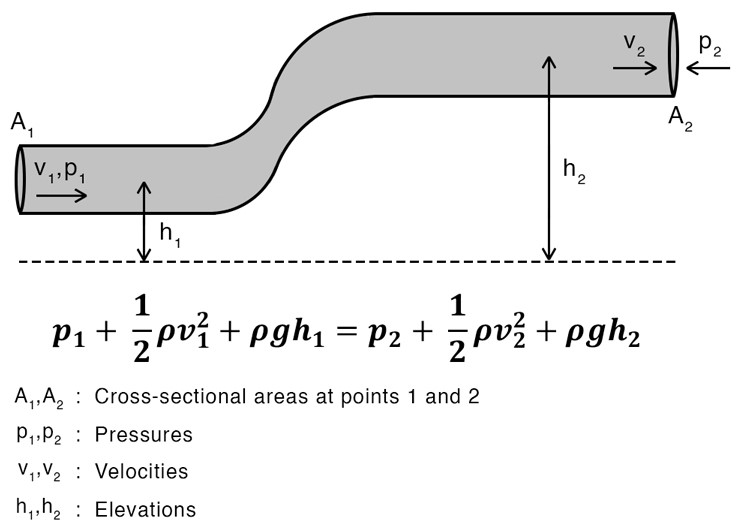
\includegraphics[scale=0.55]{Bernoullis.jpg}
    \caption{Bernoulli's Theorem}
\end{figure}
\subsection*{Applications of Bernoulli's principle}
\begin{itemize}
  \item The Bernoulli equation can be applied to devices such as the orifice meter, Venturi meter, and Pitot tube and which are used to measure flow in open channels and tubes.
  \item The Bernoulli equation can be used to calculate the lift generated by the wing of an aeroplane.\\
\end{itemize}

\subsection*{Reason behind choosing this equation}
I chose Bernoulli's principle because it is a fundamental concept in fluid dynamics, which plays a crucial role in the field of aerospace engineering. As an aspiring aerospace engineer, understanding how fluids behave and interact with objects is essential for designing efficient aircraft and spacecraft. Bernoulli's principle provides insights into the relationship between fluid pressure, velocity, and elevation.

\bibliography{refs}
\bibliographystyle{alpha}
\end{document}
